% $Header: /Users/paul/Classes/8220/Presentation/RCS/route-recovery.tex,v 1.1 2009/04/17 07:03:56 paul Exp $

\documentclass{beamer}

% This file is a solution template for:

% - Giving a talk on some subject.
% - The talk is between 15min and 45min long.
% - Style is ornate.



% Copyright 2004 by Till Tantau <tantau@users.sourceforge.net>.
%
% In principle, this file can be redistributed and/or modified under
% the terms of the GNU Public License, version 2.
%
% However, this file is supposed to be a template to be modified
% for your own needs. For this reason, if you use this file as a
% template and not specifically distribute it as part of a another
% package/program, I grant the extra permission to freely copy and
% modify this file as you see fit and even to delete this copyright
% notice. 


\mode<presentation>
{
  \usetheme{Frankfurt}
  % or ...
  
  \setbeamercovered{transparent}
  % or whatever (possibly just delete it)

  \usefonttheme[onlymath]{serif}
  
}
\documentclass[conference, 11pt]{IEEEtran} 
\usepackage{verbatim}
\usepackage{multirow} \usepackage{enumerate}
\usepackage{amsmath,enumerate} \usepackage{amsthm}
\usepackage{algcompatible}
\usepackage{algpseudocode}
\usepackage{algorithm}
%\usepackage{algorithmic}
\usepackage{pstricks}
\usepackage{amssymb, latexsym}
\usepackage{xfrac}
\usepackage{mathtools}
\usepackage{graphicx}
\usepackage{subfig}
\DeclareGraphicsRule{*}{mps}{*}{}
\usepackage{listings}

%specific to this document only
\usepackage{pgfplots}
\usepackage{pgfplotstable}
\pgfplotstableread{plts/experiment8b1_av.tab}\averageone
\pgfplotstableread{plts/experiment8b2_av.tab}\averagetwo
\pgfplotstableread{plts/experiment8b3_av.tab}\averagethree
\pgfplotstableread{plts/experiment8b4_av.tab}\averagefour
\pgfplotstableread{plts/experiment9a_av.tab}\stepping
\pgfplotstableread{plts/experiment9a1_av.tab}\steppingone
\pgfplotstableread{plts/experiment9a2_av.tab}\steppingtwo
\pgfplotstableread{plts/experiment9a3_av.tab}\steppingthree
\pgfplotstableread{plts/experiment9a4_av.tab}\steppingfour
\pgfplotstableread{plts/experiment9b1_av.tab}\runningone
\pgfplotstableread{plts/experiment9b2_av.tab}\runningtwo
\pgfplotstableread{plts/experiment9b3_av.tab}\runningthree
\pgfplotstableread{plts/experiment9b4_av.tab}\runningfour
\pgfplotstableread{plts/experiment9b_av.tab}\running
\pgfplotstableread{plts/experiment9c_av.tab}\costcomp
\pgfplotstableread{plts/experiment9c1_av.tab}\costcompone
\pgfplotstableread{plts/experiment9c2_av.tab}\costcomptwo
\pgfplotstableread{plts/experiment9c3_av.tab}\costcompthree
\pgfplotstableread{plts/experiment8b1_rn.tab}\runsone
\pgfplotstableread{plts/experiment8b2_rn.tab}\runstwo
\pgfplotstableread{plts/experiment8b3_rn.tab}\runsthree
\pgfplotstableread{plts/experiment8b4_rn.tab}\runsfour
\pgfplotstableset{
  create on use/density/.style={
    create col/expr={\thisrow{nodes}+\thisrow{links}}}
    }
\pgfplotstableset{
  create on use/delta/.style={
    create col/expr={\thisrow{links}*2}}
    }
\pgfplotstableset{
  create on use/nodebylinks/.style={
    create col/expr={(\thisrow{nodes}*\thisrow{links})}}
    }
\pgfplotscreateplotcyclelist{three}{% 
  every mark/.append style={fill=teal}\\% 
  every mark/.append style={fill=green}\\% 
  every mark/.append style={fill=orange}\\% 
}
\pgfplotscreateplotcyclelist{four}{%
  every mark/.append style={fill=teal}\\%
  every mark/.append style={fill=green}\\%
  every mark/.append style={fill=orange}\\%
  every mark/.append style={fill=pink}\\%
}

%%%%%%%%%%%%%

\usepackage{pgf}
\usepackage{tikz}
\usetikzlibrary{decorations.pathmorphing} % LATEX and plain TEX when using Tik Z
\usetikzlibrary{positioning}
\usetikzlibrary{er}
\usetikzlibrary{automata}
\usetikzlibrary{shapes.geometric}
\tikzstyle{vx}=[draw,circle,fill=white,minimum size=2pt, inner sep=1pt, node distance=15mm]
\tikzstyle{ex}=[draw,rectangle,fill=white,minimum size=2pt, inner sep=3pt, node distance=15mm]
\tikzstyle{bup}=[semithick, decoration={bent, aspect=.3, amplitude=4}, decorate, ->, >=stealth]
\tikzstyle{bdn}=[semithick, decoration={bent, aspect=.3, amplitude=-4}, decorate, ->, >=stealth]
\tikzstyle{BUP}=[thick, decoration={bent, aspect=.3, amplitude=8}, decorate, ->, >=stealth]
\tikzstyle{BDN}=[thick, decoration={bent, aspect=.3, amplitude=-8}, decorate, ->, >=stealth]
\tikzstyle{MUP}=[thick, decoration={bent, aspect=.3, amplitude=16}, decorate, ->, >=stealth]
\tikzstyle{MDN}=[thick, decoration={bent, aspect=.3, amplitude=-16}, decorate, ->, >=stealth]
\tikzstyle{str}=[semithick, decorate, ->, >=stealth]
\tikzstyle{cr}=[draw, circle, fill=black!25,minimum size=150pt]

%styles for plots?
\tikzstyle{bls}=[blue, solid, mark=square*]
\tikzstyle{grt}=[red, solid, mark=*]
% \paperheight=11in \paperwidth=8.5in \textheight=9.0in
% \textwidth=6.5in \voffset=-.875in \hoffset=-.875in
\newenvironment{code} {\begin {quote}\begin{footnotesize}}
    {\end{footnotesize}\end{quote}}

% \oddsidemargin 0.0 in \evensidemargin 0.0 in
\newenvironment{enumeratealpha}
{\begin{enumerate}[(a{\textup{)}}]}{\end{enumerate}}

\theoremstyle{plain}
\newtheorem{lem-rule}{Rule}
\newtheorem{thm}{Theorem}
\newtheorem{lem}{Lemma}[thm]
\newtheorem{prop}{Proposition}[thm]
\newtheorem{lprp}{Proposition}[lem]
\theoremstyle{definition}
\newtheorem{defn}{Definition}[thm]
\newtheorem{dfn}{Definitions}[thm]
\newtheorem{ldef}{Definition}
\theoremstyle{remark}
\newtheorem{smy}{Summary}
\newtheorem{note}{Note}[thm]

%algorithms commands
\algblockdefx[Case]{Case}{EndCase} %
[1] [{\em var}] {{\bfseries case} {\em #1\ } } %
{{\bfseries end case}}%
\algcblockdefx[Case]{Case}{When}{EndCase}
[1] [{\em true}] {{\bfseries when} {\em #1\ }}
{{\bfseries end case}} %

\algblockdefx[TimesDo] {DoTimes}{EndTimes}
[1] [0] {#1 times {\bfseries do}}
{{\bfseries end do}}

%subalgorithms environment
\makeatletter
\newcounter{parentalgorithm}
\newenvironment{subalgorithms}{%
%  \refstepcounter{algorithm}%
  \floatname{algorithm}{Procedure}
  \protected@edef\theparentalgorithm{\thealgorithm}%
  \setcounter{parentalgorithm}{\value{algorithm}}%
  \setcounter{algorithm}{0}%
  \def\thealgorithm{\theparentalgorithm-\alph{algorithm}}%
  \ignorespaces
}{%
  \setcounter{algorithm}{\value{parentalgorithm}}%
  \ignorespacesafterend
}
\makeatother

%code environments
\usepackage{float}
 
\floatstyle{ruled}
\newfloat{codeblock}{thp}{lop}
\floatname{codeblock}{Example}

\lstnewenvironment{rubyblock} 
{\lstset{language=Ruby, basicstyle=\small, xleftmargin=10pt, numbers=left, numberstyle=\tiny, stepnumber=2, numbersep=5pt}}
{}
% text macros
\def\cI{{\mathcal I}} \def\cR{{\mathcal R}} \def\cE{{\mathcal E}}
\def\cC{{\mathcal C}} \def\cF{{\mathcal F}} \def\cU{{\mathcal U}}
\def\cH{{\mathcal H}} \def\cD{{\mathcal D}} \def\cB{{\mathcal B}}
\def\cQ{{\mathcal Q}} \def\cV{{\mathcal V}} \def\cS{{\mathcal S}}
\def\cG{{\mathcal G}} \def\cA{{\mathcal A}} \def\cO{{\mathcal O}}
\def\cW{{\mathcal W}} \def\cL{{\mathcal L}} 

\def\bI{{\mathbb I}} \def\bO{{\mathbb O}}
\def\bC{{\mathbb C}} \def\bM{{\mathbb M}}
\def\bId{{$\mathbb I$}} \def\bOd{{$\mathbb O$}}
\def\bCd{{$\mathbb C$}} \def\bMd{{$\mathbb M$}}

\def\cId{{$\mathcal I$}} \def\cRd{{$\mathcal R$}} \def\cEd{{$\mathcal E$}} 
\def\cCd{{$\mathcal C$}} \def\cFd{{$\mathcal F$}} \def\cUd{{$\mathcal U$}} 
\def\cHd{{$\mathcal H$}} \def\cDd{{$\mathcal D$}} \def\cBd{{$\mathcal B$}} 
\def\cQd{{$\mathcal Q$}} \def\cVd{{$\mathcal V$}} \def\cSd{{$\mathcal S$}} 
\def\cGd{{$\mathcal G$}} \def\cAd{{$\mathcal A$}} \def\cOd{{$\mathcal O$}}
\def\cWd{{$\mathcal W$}} \def\cLd{{$\mathcal L$}}

\bibliographystyle {IEEEtranS}

\usepackage[english]{babel}
% or whatever

\usepackage[latin1]{inputenc}
% or whatever

\usepackage{times}
\usepackage[T1]{fontenc}
\usepackage{graphics}
% Or whatever. Note that the encoding and the font should match. If T1
% does not look nice, try deleting the line with the fontenc.

% le bib style
\bibliographystyle {IEEEtranS}

\title[Distributed MWVC in Random Graphs] % (optional, use only with long paper titles)
{Distributed Vertex Cover in Random Networks with Applications to the Network Lifetime Problem}

\subtitle
{Project in Fulfillment of Masters Degree} % (optional)

\author[] % (optional, use only with lots of authors)
{John P. Daigle}
% - Use the \inst{?} command only if the authors have different
%   affiliation.

\institute[Georgia State University] % (optional, but mostly needed)
{
  Department of Computer Science\\
  Georgia State University}

% - Use the \inst command only if there are several affiliations.
% - Keep it simple, no one is interested in your street address.

\date[] % (optional)
{04.17.09}

\subject{Talks}
% This is only inserted into the PDF information catalog. Can be left
% out. 



% If you have a file called "university-logo-filename.xxx", where xxx
% is a graphic format that can be processed by latex or pdflatex,
% resp., then you can add a logo as follows:

% \pgfdeclareimage[height=0.5cm]{university-logo}{university-logo-filename}
% \logo{\pgfuseimage{university-logo}}



% Delete this, if you do not want the table of contents to pop up at
% the beginning of each subsection:
\AtBeginSection[]
{
  \begin{frame}<beamer>
    \frametitle{Outline}
    \tableofcontents[currentsection,currentsubsection]
  \end{frame}
}


% If you wish to uncover everything in a step-wise fashion, uncomment
% the following command: 

%\beamerdefaultoverlayspecification{<+->}


\begin{document}

\begin{frame}
  \titlepage
\end{frame}

\begin{frame}
  \frametitle{Outline}
  \tableofcontents
  % You might wish to add the option [pausesections]
\end{frame}

\section{Introduction}
\begin{frame}
  \frametitle{Definitions}
  \begin{block}{Vertex Disjoint}
    Two paths are point/node/vertex disjoint if they have common endpoints but no common midpoints.
  \end{block}
  \begin{center}
    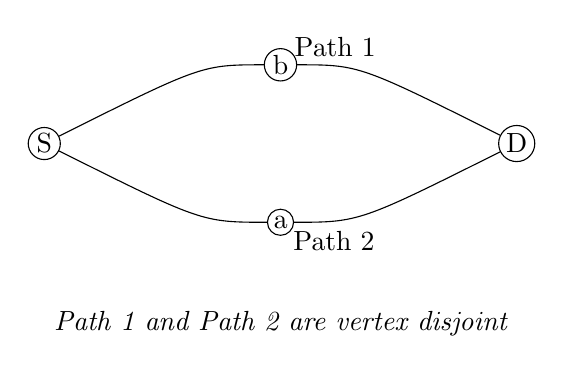
\begin{tikzpicture}
      \node [vx](s) at (0,1) {S};
      \node [vx] (m1) at (3,0) {a};
      \node [vx] (d) at (6,1) {D};
      \node [vx] (m2) at (3,2) {b};
      \draw [rounded corners] (s) .. controls (2,0) .. (m1) .. controls (4,0) .. (d) coordinate [near start, label=below:Path 2, ] {};
      \draw (s) .. controls (2,2) .. (m2) .. controls (4,2) .. (d) coordinate [near start, label=above:Path 1];
\node [below=1cm ] at (m1) {{\em Path 1 and Path 2 are vertex disjoint}};
    \end{tikzpicture}
\end{center}
\end{frame}

\begin {frame}
  \frametitle{Relevance}
  \begin{block}{Multi-Path routing}
    A routing scheme in which a given source has two or more paths to a destination is a {\em Multi-path} scheme. If those paths are strictly vertex disjoint, there are benefits in load balancing, QoS, and redundancy.
  \end{block}
\end{frame}

\begin {frame}
  \frametitle{Research Questions}
  \begin{enumerate}
  \item When one of a set of $N$ \vdps\ is broken due to a node failure or linkage failure, is it possible to create a new set of $N$ \vdps ?
  \item If a set of $N$ \VDPs\ cannot be created, is it possible to determine the correct position for some nodes to take in order to create the set?
  \item What information is needed to compute a set of $N$ \VDPs, and how can this be accomplished using only local information?
  \end{enumerate}

  \begin{block}{Goal}
    The authors goal is to implement a distributed algorithm that allows a network to maintain a minimum number of vertex disjoint paths from any source to a specific destination.
  \end{block}
\end{frame}

\begin{frame}
  \frametitle{Claims}
  The authors make three basic claims.
  \begin{enumerate}
  \item They identify the conditions in which a vertex disjoint path exists
  \item They provide a maintenance framework for cases in which a minimum number of {\bf VDPs} are required but some may be lost over time
  \item They argue that this algorithm is a good complement for traditional max-flow algorithms in cases where {\bf VDPs} are required.
  \end{enumerate}
\end{frame}

\section{Path Existence}
\subsection{Flip Algorithm}

\begin{frame}
  \frametitle{Notation}
  \begin{tabular}{|c|p{22em}|}
    \hline
    $S$&$S$ is the source node of the basic set\\
    \hline
    $P$&$P$ is the source node of the reference set.\\ 
    \hline
    $T$&$T$ is the destination node.\\
    \hline
    $\cC_S$&$\cC_S = \{S_{T_1} , S_{T_2} ,\dots, S_{T_i} ,\dots, S_{T_{N_B}} \}$, the basic set, where $N_B$ is the number of paths and $1 \le i \le N_B$.\\
    \hline
    $\cC_P$& $\cC_P = \{P_{T_1} , P_{T_2} ,\dots, P_{T_j} ,\dots, P_{T_{N_R}} \}$, the reference set, where $N_R$ is the number of paths and $1 \le j \le N_R$ .\\
    \hline
    $S_{T_i}$&$S_{T_i} = \{s_{i_0} , s_{i_1} ,\dots, s_{i_{B_i}} \}$, the ith path in the basic set, where $s_{i_0}= S$, $s_{i_{B_i}} = T$ and $B_i$ is the number of vertexes.\\
    \hline
    $P_{T_j}$ & $P_T= \{p_{j_0} , p_{j_1} ,\dots, p_{j_{R_j}}\}$, the $jth$ path in the reference set, where $p_{j_0} = P$, $p_{j_{R_j}}= T$ and $R_j$ is the number of vertexes. \\
    \hline
  \end{tabular}
  
\end{frame}
\begin{frame}
  \frametitle{First Level Induced Path}
  \begin{block}{Paired Vertex Disjoint Set}
    Given a source node and a destination node $(S,D)$, a set of \vdps\ between them is a paired vertex disjoint path set *(My Notation)
  \end{block}
  \begin{block}{Induced Path}
    Given two sources ($S,P$) and one destination $D$, where one source $S$ is designated as the basic source and one source $P$, as the reference source, an induced path is a path that starts at $S$, overlaps {\bf exactly} one path in the basic set $\cC_S$, overlaps {\em at most} one path in the reference set $\cC_P$, and ends at $D$. 
  \end{block}
\end{frame}

\begin{frame}
\frametitle{Example of an Induced Path}
\begin{center}
\begin{tikzpicture}
    \useasboundingbox (4,0) rectangle (4,0);
      \node [vx](s) {$S$};
      \node [vx](r) [below right=of s] {$R$};
      \node [vx](a1) [above right=of s] {$a_1$};
      \node [vx](a2) [right=of a1] {$a_2$};
      \node [vx](a3) [right=of a2] {$a_3$};
      \node [vx](a4) [right=of s]{$a_4$};
      \node [vx](a5) [right=of a4]{$a_5$};
      \node [vx](a6) [right=of a5]{$a_6$};
      \node [vx](b1) [below right=of r] {$b_1$};
      \node [vx](b2) [right=of b1] {$b_2$};
      \node [vx](b3) [right=of b2] {$b_3$};
      \node [vx](b4) [right=of r] {$b_4$};
      \node [vx](b5) [right=of b4] {$b_5$};
      \node [vx](b6) [right=of b5] {$b_6$};
      \node [vx](d) [right=of b6] {$D$};
      \draw <1,3->[bup](s) --  (a1) -- (a2) to (a3) to (d) [red];
      \draw <1,3->[bup](s) to (a4) to (a5) to (a6) to (d) [red];
      \draw <1,3->[bdn](s) to (b4) to (b5) to (b6) to (d) [red];
      \draw <2->[bup](r) to (b1) to (b2) to (b3) to (d) [green, bend left, ->];
      \draw <2->[bup](r) to (b4) to (b5) to (b6) to (d) [green, ->];
      \draw <3>[bdn](s) to (a4) to (b1) to (b2) to (b3) to (d) [blue, bend right, ->, >=stealth];
      \node <1>[right=1cm ] at (a3) {$\cC_s$};
      \node <2>[above=1cm ] at (b6) {$\cC_P$};
      \node <3>[above=1cm] at (a2) {An induced path on Basic Set $\cC_S$, and  Reference Set $\cC_P$};
\end{tikzpicture}
\end{center}
\end{frame}

\begin{frame}
  \frametitle{The Ordered Intersection Set}
  \begin{block}{Definition}
    $X_i = \{S_{i_k} | \exists j, S_T.s_{i_k} \in P_{T_j},0 \leq k \leq B_i\}$ is the ordered intersection set of $S_{T_i}$. A vertex is a member of $X_i$ if it is on a specific path $S_{T_i}$ and a path $P_{T_j}$ in $cC_P$.

    The set is ordered because for each $s_{i_n}, S_{i_m}$ in $X_i$, $n < m$ if $s_{i_n}$ can reach $S$ in fewer hops than $s_{i_m}$
    
  \end{block}
\end{frame}

\begin{frame}
  \frametitle{Example of an Ordered Intersection Set}
  \begin{center}
    \begin{tikzpicture}
      \useasboundingbox (4,0) rectangle (4,0);
      \node [vx](s) {$S$};
      \node [vx](r) [below right=of s] {$R$};
      \node [vx](a1) [above right=of s] {$a_1$};
      \node [vx](a2) [right=of a1] {$a_2$};
      \node [vx](a3) [right=of a2] {$a_3$};
      \node [vx](a4) [right=of s]{$a_4$};
      \node [vx](a5) [right=of a4]{$a_5$};
      \node [vx](a6) [right=of a5]{$a_6$};
      \node [vx](b1) [below right=of r] {$b_1$};
      \node [vx](b2) [right=of b1] {$b_2$};
      \node [vx](b3) [right=of b2] {$b_3$};
      \node [vx](b4) [right=of r] {$b_4$};
      \node [vx](b5) [right=of b4] {$b_5$};
      \node [vx](b6) [right=of b5] {$b_6$};
      \node [vx](d) [right=of b6] {$D$};
      \draw <1>[bup](s) --  (a1) -- (a2) to (a3) to (d) [red];
      \draw <1>[bup](s) to (a4) to (a5) to (a6) to (d) [red];
      \draw <1>[bdn](s) to (b4) to (b5) to (b6) to (d) [red];
      \draw <1->[bup](r) to (b1) to (b2) to (b3) to (d) [green];
      \draw <1->[bup](r) to (b4) to (b5) to (b6) to (d) [green];
    \end{tikzpicture}
  \end{center}
\end{frame}



\begin{frame}
  \frametitle{Flip Algorithm}
  \small{
    \begin{algorithmic}
      \STATE Construct the ordered intersection set for each path in $C_S$
      \IF {$\exists i, s.t. X_i = \emptyset$}
      \STATE $S_{T_i}$ is the induced path
      \STATE STOP
      \ENDIF
      \STATE Find the effective partition nodes for each path in $C_P$
      \STATE Set $l = 1$
      \LOOP
      \IF {$\exists i, s.t. S_{T_i}$'s $l$th level subpath joints an effective residual path of $P_{T_j}$}
      \STATE The induced path is the concatenation of these two subpaths
      \STATE STOP
      \ENDIF
      \STATE $l=l+1$
      \ENDLOOP
    \end{algorithmic}
  }
\end{frame}

\begin{frame}
  \frametitle{Concept}
\end{frame}

\subsection{Omvdp Algorithm}
\begin{frame}
\end{frame}
\begin{frame}
  \frametitle{Notation}
  \begin{tabular}{|c|p{22em}|}
    \hline
    $A$&$A = \{S_{T_1}, S_{T_2},\dots, S_{T_i},\dots, S_{T_N-1}\}$, the set of vertex-disjoint paths for the $(N-1)$-credit node $S$ is the source node of the basic set\\
    \hline
    $B$&$B = \{P_{T_1} , P_{T_2} ,\dots, P_{T_j} ,\dots, P_{T_N} \}$, the set of vertex-disjoint paths for the $N$-credit node $P$ \\ 
    \hline
    $New_A$&$New_A = NewA = \{new_1 , new_2 ,\dots, new_N \},$,  the set of vertex-disjoint paths constructed by Omvdp for $S$\\
    \hline
  \end{tabular}
\end{frame}

\begin{frame}[allowframebreaks]
\frametitle{Algorithm}
\begin{algorithmic}
  \STATE $C_S \leftarrow A$, $C_P \leftarrow B$, $New_A \leftarrow \emptyset$
\end{algorithmic}
\end{frame}


\section{Route Recovery}
\section{With Max-Flow}

\section{Bibliography}
\begin{frame}
\frametitle{Bibliography}
\bibliography{vertex_bib.bib}
\end{frame}
\end{document}
